\documentclass[twoside]{article} \usepackage{aistats2017}

% If your paper is accepted, change the options for the package
% aistats2017 as follows:
%
%\usepackage[accepted]{aistats2017}
%
% This option will print headings for the title of your paper and
% headings for the authors names, plus a copyright note at the end of
% the first column of the first page.

\bibliographystyle{apalike}  % Use the "unsrtnat" BibTeX style for formatting the Bibliography
\usepackage[square, authoryear, comma, sort&compress]{natbib}  % Use the "Natbib" style for the references in the Bibliography

\usepackage{amsmath}
\usepackage{amssymb}
\usepackage{amsthm}
\usepackage{mathbbol}
\usepackage{mathtools}
\usepackage{mathrsfs}
\usepackage{bm}
\usepackage{vector}
\usepackage[usenames, dvipsnames]{color}
\usepackage{cleveref}
\usepackage{graphicx}
\usepackage{caption}
\usepackage{subcaption}

\theoremstyle{definition}
\newtheorem{theorem}{Theorem}[section]
\newtheorem{corollary}[theorem]{Corollary}
\newtheorem{definition}[theorem]{Definition}
\newtheorem{lemma}[theorem]{Lemma}
\newtheorem{identity}[theorem]{Identity}

\newcommand{\eq}[1]{\begin{equation} \begin{aligned} #1 \end{aligned} \end{equation}}

\newcommand{\argmin}{\operatornamewithlimits{argmin}}
\newcommand{\rv}[1]{{#1}}
\newcommand{\ds}[1]{\tilde{#1}}
\newcommand{\warn}[1]{{\color{red} #1}}
\newcommand{\extra}[1]{{\color{ForestGreen} #1}}
\newcommand{\qpi}{QPI }

\newcommand{\expect}[1]{{\mathbb{E}[#1]}}
\newcommand{\inner}[2]{{\langle #1, #2 \rangle}}

\newcommand{\Hk}{\mathcal{H}_{k}}
\newcommand{\Hl}{\mathcal{H}_{l}}
\newcommand{\muX}{\mu_{\rv{X}}}
\newcommand{\muY}{\mu_{\rv{Y}}}
\newcommand{\muYx}{\mu_{\rv{Y} | \rv{X} = x}}
\newcommand{\muXy}{\mu_{\rv{X} | \rv{Y} = y}}
\newcommand{\phiX}{\phi_{\rv{X}}}
\newcommand{\psiY}{\psi_{\rv{Y}}}
\newcommand{\Cxy}{C_{\rv{X} \rv{Y}}}
\newcommand{\Cyx}{C_{\rv{Y} \rv{X}}}
\newcommand{\Cxx}{C_{\rv{X} \rv{X}}}
\newcommand{\Cyy}{C_{\rv{Y} \rv{Y}}}
\newcommand{\Cylx}{C_{\rv{Y} | \rv{X}}}
\newcommand{\Cxly}{C_{\rv{X} | \rv{Y}}}

\newcommand{\hatmuX}{\hat{\mu}_{\rv{X}}}
\newcommand{\hatmuY}{\hat{\mu}_{\rv{Y}}}
\newcommand{\hatmuYx}{\hat{\mu}_{\rv{Y} | \rv{X} = x}}
\newcommand{\hatmuXy}{\hat{\mu}_{\rv{X} | \rv{Y} = y}}
\newcommand{\hatCxy}{\hat{C}_{\rv{X} \rv{Y}}}
\newcommand{\hatCyx}{\hat{C}_{\rv{Y} \rv{X}}}
\newcommand{\hatCxx}{\hat{C}_{\rv{X} \rv{X}}}
\newcommand{\hatCyy}{\hat{C}_{\rv{Y} \rv{Y}}}
\newcommand{\hatCylx}{\hat{C}_{\rv{Y} | \rv{X}}}
\newcommand{\hatCxly}{\hat{C}_{\rv{X} | \rv{Y}}}
\newcommand{\cardX}{\Vert \mathcal{X} \Vert}
\newcommand{\cardY}{\Vert \mathcal{Y} \Vert}

\begin{document}

% If your paper is accepted and the title of your paper is very long,
% the style will print as headings an error message. Use the following
% command to supply a shorter title of your paper so that it can be
% used as headings.
%
%\runningtitle{I use this title instead because the last one was very long}

% If your paper is accepted and the number of authors is large, the
% style will print as headings an error message. Use the following
% command to supply a shorter version of the authors names so that
% they can be used as headings (for example, use only the surnames)
%
%\runningauthor{Surname 1, Surname 2, Surname 3, ...., Surname n}

\twocolumn[

\aistatstitle{Quantile Regression with Kernel Embeddings}

\aistatsauthor{ Anonymous Author 1 \And Anonymous Author 2 \And Anonymous Author 3 }

\aistatsaddress{ Unknown Institution 1 \And Unknown Institution 2 \And Unknown Institution 3 } ]

\begin{abstract}
  The Abstract paragraph should be indented 0.25 inch (1.5 picas) on
  both left and right-hand margins. Use 10~point type, with a vertical
  spacing of 11~points. The {\bf Abstract} heading must be centered,
  bold, and in point size 12. Two line spaces precede the
  Abstract. The Abstract must be limited to one paragraph.
\end{abstract}

\warn{Red lines are notes to pay attention to. They are not part of the paper.}

\extra{Green lines are sections that we are considering to delete. They are part of the paper.}

\section{Introduction}
\label{sec:introduction}
	
	\warn{Why quantile regression? What are the advantages of quantile regression over regular regression?}
	
	Understanding risk is critical to making decisions based on uncertain information. Computing uncertainty through the use of probability, and then bounding that uncertainty with quantile estimation is one approach to this problem. Building from our work in chapter three, we now aim to extend our non-parametric, multi-modal techniques for regression to include cumulative and quantile estimation. With these additions, our work can be applied to problems with unknown prior and likelihood and produce not only probabilistic estimations, but also quantify the risk associated with decisions that rely on them.
	
%	\begin{figure}
%		\begin{center}
%			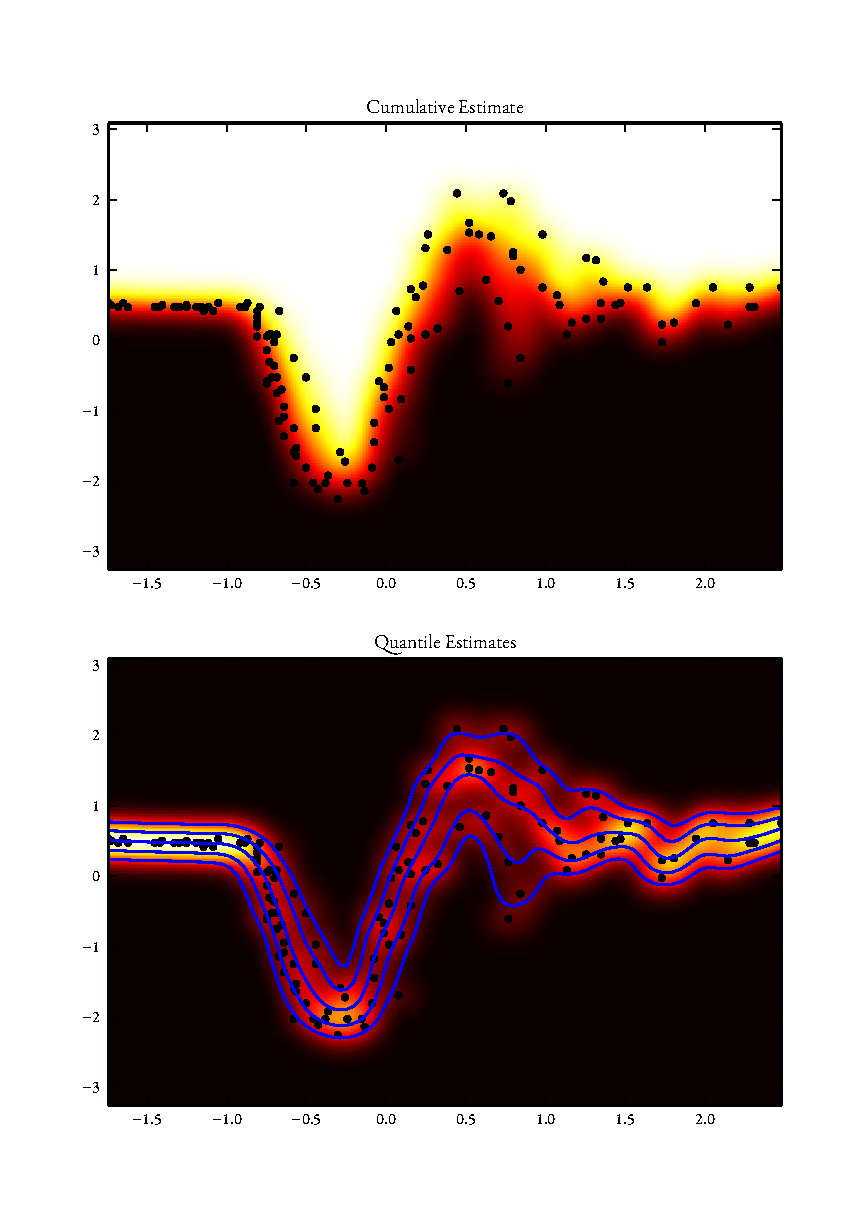
\includegraphics[width=\columnwidth]{figures/mcquantiles}
%		\end{center}
%		\caption{\small Estimate of the cumulative embedding (top),
%			and the quantiles 0.1, 0.25, 0.5, 0.75, 0.9 overlaying a PDF estimate
%			(bottom)}
%		\label{fig:cembedding}
%	\end{figure}

	\begin{figure}
		\begin{center}
			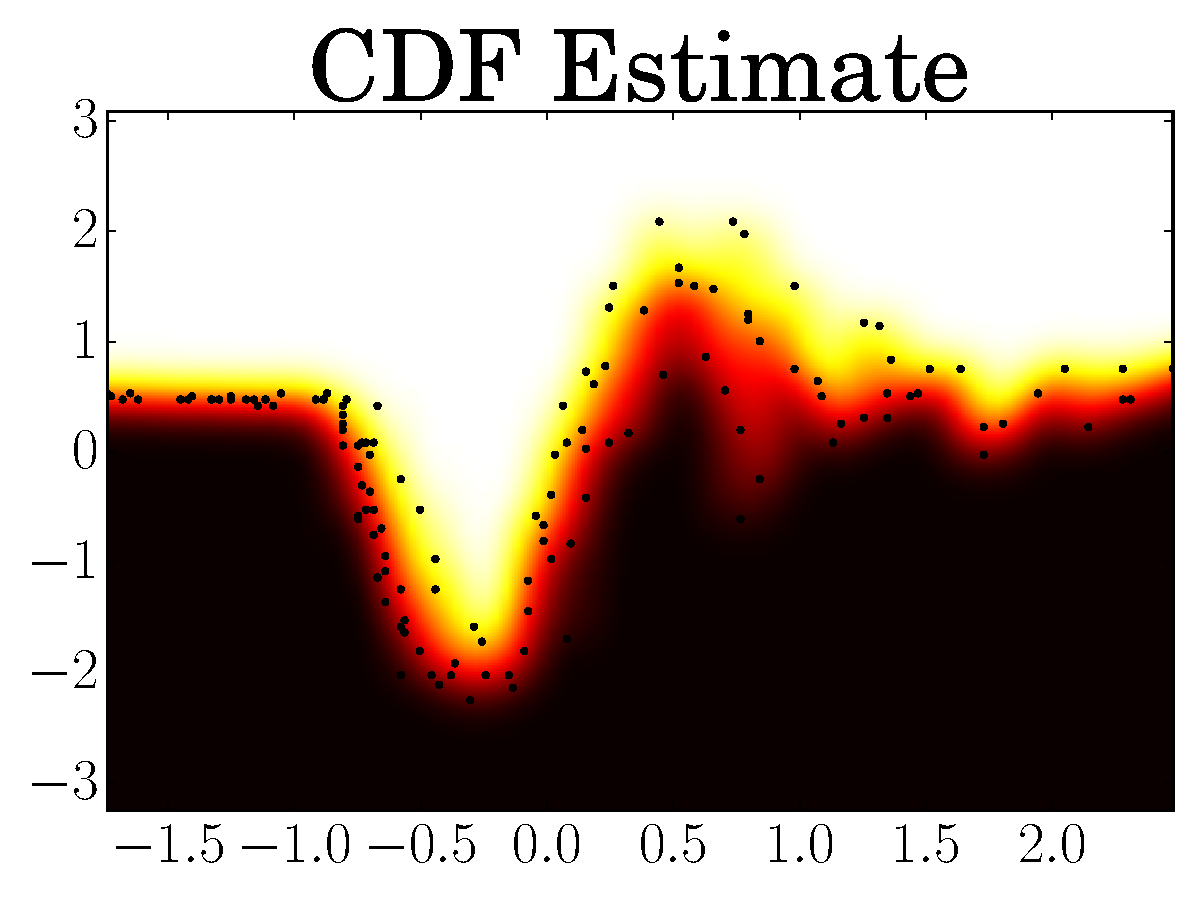
\includegraphics[width=0.48\columnwidth]{figures/mcquantiles_1}
			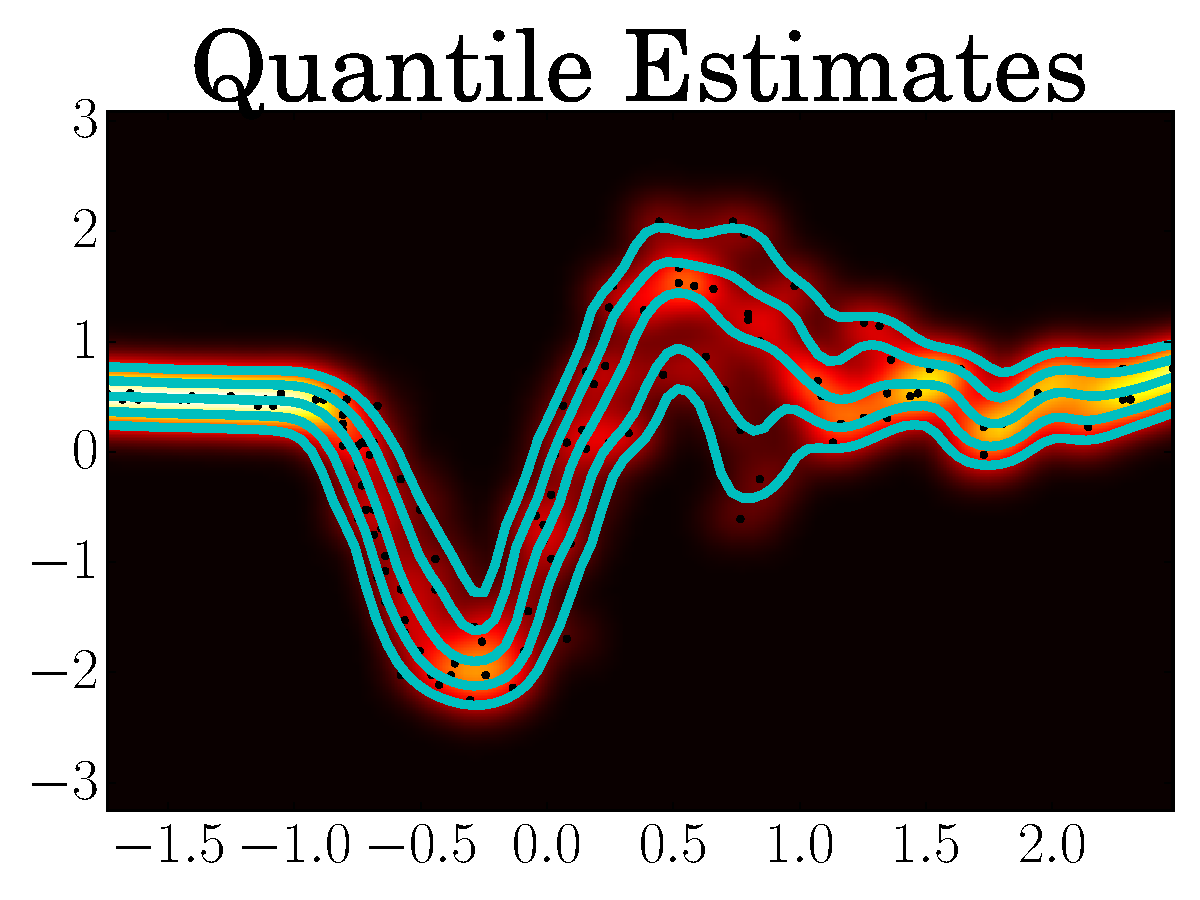
\includegraphics[width=0.48\columnwidth]{figures/mcquantiles_2}
		\end{center}
		\caption{\small Estimate of the cumulative embedding (top),
			and the quantiles 0.1, 0.25, 0.5, 0.75, 0.9 overlaying a PDF estimate
			(bottom)}
		\label{fig:cembedding}
	\end{figure}
	
	\warn{Not done yet. Come back later.}
	
\section{Background}
\label{sec:background}
	
	\warn{This section is taken from the supplementary materials. Only the relevant bits are taken. The point is to have an expanded version of the background in the supplementary. We do want this to be at least one page just for kernel embeddings.}
	
	Let $(\Omega, \mathcal{W}, \mathbb{P})$ be a probability space, where $\Omega$ is the sample space, $\mathcal{W}$ is a $\sigma$-algebra on $\Omega$, and $\mathbb{P} : \mathcal{W} \mapsto [0, 1]$ a probability measure. The elements $W$ of $\mathcal{W}$, that is, the measurable sets, are called events, which are by definition subsets of $\Omega$.
	
	\begin{definition} \label{def:distribution}
		(Distribution)
		The \textit{distribution} of a random variable $\rv{X} : \Omega \mapsto \mathcal{X}$ is the Borel measure $\mathbb{P}_{\rv{X}} : \mathcal{A} \mapsto [0, 1]$ defined by
		\begin{equation}
			\mathbb{P}_{\rv{X}}[A] := \mathbb{P}[\rv{X} \in A]
		\label{eq:distribution}
		\end{equation}
		where the event $\{\rv{X} \in A\} := \rv{X}^{-1}[A] := \{\omega \in \Omega : \rv{X}(\omega) \in A\} \in \mathcal{W}$ is the inverse image (pre-image) of $A \subseteq \mathcal{X}$ under the random variable $\rv{X}$, and $\mathcal{A}$ is a $\sigma$-algebra of subsets on $\mathcal{X}$.
	\end{definition}
	
	\begin{definition} \label{def:cdf}
		(Cumulative Distribution Function)
		The \textit{cumulative distribution function} (CDF) $P_{\rv{X}} : \mathbb{R} \mapsto [0, 1]$ of a \textit{real-valued} random variable $\rv{X} : \Omega \mapsto \mathbb{R}$ and random vector $\bvec{\rv{X}} : \Omega \mapsto \mathbb{R}^{d}$ is defined as follows \eqref{eq:cdf}.
		\begin{equation}
			\begin{aligned}
				P_{\rv{X}}(x) &:= \mathbb{P}_{\rv{X}}[(-\infty, x]] = \mathbb{P}[\rv{X} \leq x] \\
				P_{\bvec{\rv{X}}}(\bvec{x}) &:= \mathbb{P}_{\bvec{\rv{X}}}[(-\infty, x_{1}] \times \dots \times (-\infty, x_{d}]] = \mathbb{P}[\bvec{\rv{X}} \leq \bvec{x}] \\
			\end{aligned}
		\label{eq:cdf}
		\end{equation}

		For conciseness, we define the following shorthand \eqref{eq:shorthand}. 
		\begin{equation}
			\begin{aligned}
				\{\rv{X} \leq x\} &:= \{\rv{X} \in (-\infty, x]\} \\
				\{\bvec{\rv{X}} \leq \bvec{x}\} &:= \bigcap\limits_{j = 1}^{d} \{\rv{X}_{j} \in (-\infty, x_{j}]\} \in \mathcal{W} \\
				(-\bvec{\infty}, \bvec{x}] &:= (-\infty, x_{1}] \times \dots \times (-\infty, x_{d}] \\
			\end{aligned}
		\label{eq:shorthand}
		\end{equation}
	\end{definition}
	
	\begin{theorem} \label{thm:radon_nikodym}
		(Radon-Nikodym)
		If the distribution $\mathbb{P}_{\rv{X}}$ is absolutely continuous with respect to the Lebesgue measure on $\mathcal{X} = \mathbb{R}^{d}$, then the Radon-Nikodym theorem implies the existence of a density for $\mathbb{P}_{\rv{X}}$. We call this the distribution density of $\rv{X}$, or more commonly known as the \textit{probability density function} (PDF), denoted by $p_{\rv{X}}: \mathcal{X} \mapsto [0, \infty)$.
	\end{theorem}
		
	\subsection{Kernel Embedding}
	\label{sec:background:kernel_embedding}
	
	This section summarises fundamental and important results in the field of kernel embeddings that form the background of this paper. For more detail, see the supplementary material.
	
%	\Cref{sec:background:kernel_embeddings:theoretical_representation} introduces and summarises the formulation and theory of kernel embeddings. \Cref{sec:background:kernel_embeddings:empirical_representation} then extends the theoretical work to the empirical case, focusing on representations of kernel embeddings and its structure given finite amounts of sample data.
%	
%		\subsubsection{Theoretical Representation}
%		\label{sec:background:kernel_embeddings:theoretical_representation}
%		
		In this paper we assume all kernels we deal with are positive definite and characteristic. That is, the kernel $k : \mathcal{X} \times \mathcal{X} \mapsto \mathbb{R}$ defines a unique reproducing kernel Hilbert space (RKHS), which we will denote by $\mathcal{H}_{k}$.
		
		As always, let $\rv{X} : \Omega \mapsto \mathcal{X}$ and $\rv{Y} : \Omega \mapsto \mathcal{Y}$ be a random variables with distributions $\mathbb{P}_{\rv{X}}$ and $\mathbb{P}_{\rv{Y}}$, and let $k$ and $l$ be characteristic positive definite kernels defined on $\mathcal{X}$ and $\mathcal{Y}$ respectively. Let $f \in \Hk$ and $g \in \Hl$ be real-valued functions.
		
		\begin{theorem} \label{thm:feature_functions}
			(Feature Functions)
			The feature functions that form the basis for the full RKHS are the partially applied kernels of that RKHS \eqref{eq:feature_functions}.
			\begin{equation}
				\phi_{x} := k(x, \cdot) \in \Hk ;\quad \psi_{y} := l(y, \cdot) \in \Hl
			\label{eq:feature_functions}
			\end{equation}
		\end{theorem}
		
		\begin{theorem} \label{thm:reproducing_property}
			(Reproducing Property)
			The function evaluation operator within the full RKHS is the inner product with the feature function in that RKHS \eqref{eq:reproducing_property}.
			\begin{equation}
				\inner{\phi_{x}}{f} = f(x) ;\quad \inner{\psi_{y}}{g} = g(y)
			\label{eq:reproducing_property}
			\end{equation}
			\extra{
			In particular, the kernel value between two points can be evaluated as the inner product between the feature functions at those points \eqref{eq:kernel_reproducing_property}.
			\begin{equation}
				\inner{\phi_{x}}{\phi_{x'}} = k(x, x') ;\quad \inner{\psi_{y}}{\psi_{y'}} = l(y, y')
			\label{eq:kernel_reproducing_property}
			\end{equation}
			}
		\end{theorem}
		
		\begin{definition} \label{def:kernel_embedding}
			(Kernel Embedding)
			The kernel embedding (or mean embedding) of a distribution $\mathbb{P}_{\rv{X}}$ is defined as the expectation of the corresponding feature function in that RKHS \eqref{eq:kernel_embedding}.
			\begin{equation}
				\muX \equiv \muX(\cdot) := \expect{\phiX} = \expect{k(\rv{X}, \cdot)} \in \Hk
			\label{eq:kernel_embedding}
			\end{equation}
			\extra{
			where it is understood that the $\cdot$ is a place-holder for an argument such that $\muX(\cdot) : \mathcal{X} \mapsto \mathbb{R}$ is a function and not just a value.
			}
		\end{definition}
		
		\begin{theorem} \label{thm:function_expectation}
			(Function Expectation)
			The expectation of a function of a random variable can be evaluated as the inner product between the corresponding kernel embedding and the function \eqref{eq:function_expectation}.
			\begin{equation}
				\inner{\muX}{f} = \expect{f(\rv{X})} ;\quad \inner{\muY}{g} = \expect{g(\rv{Y})}
			\label{eq:function_expectation}
			\end{equation}
		\end{theorem}
		
		
		\subsubsection{Empirical Representation}
			\label{sec:background:kernel_embeddings:empirical_representation}
			
			In practice, the actual probability distributions of interest are not available in closed form. Instead, independent and identically distributed (\textit{iid}) samples from such probability distributions are available. Suppose that joint samples $\{x_{i}, y_{i}\}_{i = 1}^{n}$ are observed and collected in an \textit{iid} fashion from the joint distribution $\mathbb{P}_{\rv{X} \rv{Y}}$. Again, let $\ds{X} := \{x_{i}\}_{i = 1}^{n}$ and $\ds{Y} := \{y_{i}\}_{i = 1}^{n}$. It is possible to represent kernel embeddings empirically such that in the limit of infinite data, the empirical representations would converge to the true representations at an appropriate rate. Most significant, however, is the fact that important results for manipulating kernel embeddings also hold for their empirical representations.
			
			\begin{theorem} \label{thm:empirical_embedding}
				(Empirical Kernel Embedding)
				The empirical representation of a kernel embedding is obtained by simply replacing the expectation with an empirical average \eqref{eq:empirical_embedding}.
				\begin{equation}
					\hatmuX = \frac{1}{n} \sum_{i = 1}^{n} \phi_{x_{i}} ;\quad \hatmuY = \frac{1}{n} \sum_{i = 1}^{n} \psi_{y_{i}}
				\label{eq:empirical_embedding}
				\end{equation}
			\end{theorem}
	
			\begin{theorem} \label{thm:empirical_function_expectation}
				(Empirical Function Expectation)
				The empirical representation of a function expectation is simply the empirical average of the function, and can be obtained by the inner product of the function with the empirical embedding \eqref{eq:empirical_function_expectation}.
				\begin{equation}
					\inner{\hatmuX}{f} = \frac{1}{n} \sum_{i = 1}^{n} f(x_{i}) ;\quad \inner{\hatmuY}{g} = \frac{1}{n} \sum_{i = 1}^{n} g(y_{i})
				\label{eq:empirical_function_expectation}
				\end{equation}
			\end{theorem}
		
%			Since the samples $\ds{X} := \{x_{i}\}_{i = 1}^{n}$ and $\ds{Y} := \{y_{i}\}_{i = 1}^{n}$ are sampled from the joint distribution $\mathbb{P}_{\rv{X} \rv{Y}}$ such that marginal samples are simply $\ds{X}$ and $\ds{Y}$ themselves, the empirical representations for regular embeddings $\muX$ and $\muY$ are easy to obtain, as per \cref{thm:empirical_embedding}.
%			
%			However, instead of a uniform average, a empirical representations of the conditional embedding would require a weighted average of the following sform \eqref{eq:empirical_conditional_embedding_form} instead.
%			
%			\begin{equation}
%			\begin{aligned}
%			\hatmuYx &= \sum_{i = 1}^{n} \alpha_{i} \psi_{y_{i}} ;\quad \hatmuXy &= \sum_{i = 1}^{n} \beta_{i} \phi_{x_{i}}
%			\label{eq:empirical_conditional_embedding_form}
%			\end{aligned}
%			\end{equation}
%			
%			where $\bm{\alpha} := \{\alpha_{i}\}_{i = 1}^{n}$ is to be determined from the samples $\ds{X}$ and $\bm{\beta} := \{\beta_{i}\}_{i = 1}^{n}$ is to be determined from the samples $\ds{Y}$.
%			
%			Before deriving the expressions for $\bm{\alpha}$ and $\bm{\beta}$ however, it is useful to introduce matrix notation for representing empirical embeddings.
%			
%			The feature functions can be viewed as an feature vector of the same dimension as the cardinality of the its domain. For example, if the domain $\mathcal{X} = \mathbb{R}^{d}$ is the $d$ dimensional euclidean space whose cardinality is uncountably infinite, then the feature function can be viewed as an uncountably infinite dimensional feature vector, indexed by the elements of $\mathcal{X} = \mathbb{R}^{d}$.
%			
%			Denote the cardinality of $\mathcal{X}$ as $\cardX$, and similarly the cardinality of $\mathcal{Y}$ as $\cardY$. With the observations $\{x_{i}, y_{i}\}_{i = 1}^{n}$ sampled from $\mathbb{P}_{\rv{X} \rv{Y}}$, there are $n$ feature vectors for each RKHS, $\{\phi_{x_{i}}\}_{i = 1}^{n}$ for $\Hk$ and $\{\psi_{y_{i}}\}_{i = 1}^{n}$ for $\Hl$. As elements within their respective RKHS for which Hilbert-Schmidt operators can operate on, $\phi_{x_{i}}$ has an effective dimension of $\cardX \times 1$ and $\psi_{y_{i}}$ has an effective dimension of $\cardY \times 1$. Since this can be said about the feature functions, which form the basis for the RKHS, this also applies to general functions within the RKHS. As such, the inner product between functions $f_{1}, f_{2} \in \Hk$ can also be written in matrix notation as $\inner{f_{1}}{f_{2}} = f_{1}^{T} f_{2}$. It can be conceptually helpful to check that $f_{1}^{T}$ is of size $1 \times \cardX$ and $f_{2}$ is of size $\cardX \times 1$ so that the result is a scalar of size $1 \times 1$.
%			
%			Recall that a matrix $A := \begin{bmatrix} \bvec{a}_{1} & \cdots & \bvec{a}_{n} \end{bmatrix} \in \mathbb{R}^{n \times n}$, $\bvec{a}_{i} \in \mathbb{R}^{n} \; \forall i \in \{1, \dots, n\}$, operated on a vector $\bvec{v} \in \mathbb{R}^{n}$ results in a vector that is the linear combination of the columns of $A$ with coefficients given by the components of $\bvec{v}$. That is, $A \bvec{v} = \sum_{i = 1}^{n} v_{i} \bvec{a}_{i}$.
%			
%			Similarly, a feature matrix can be defined in the same way such that empirical representations of kernel embeddings can be reduced down to linear algebraic operations.
%			
			\begin{definition} \label{def:feature_matrix}
				(Feature Matrix)
				A feature matrix $\Phi \equiv \Phi_{\ds{X}}$ is formed by stacking the corresponding feature vectors \textit{horizontally}, where each feature vector represents a column of that matrix \eqref{eq:feature_matrix}. Here, the subscripts of $\Phi$ and $\Psi$ are dropped whenever it is clear from context the dataset involved. In this way, $\Phi$ has effective size $\cardX \times n$ and $\Psi$ has effective size $\cardY \times n$.	
				
				\begin{equation}
					\Phi := \begin{bmatrix} \phi_{x_{1}} & \cdots & \phi_{x_{n}} \end{bmatrix}; \quad
					\Psi := \begin{bmatrix} \psi_{y_{1}} & \cdots & \psi_{y_{n}} \end{bmatrix}
				\label{eq:feature_matrix}
				\end{equation}
				
		
			\end{definition} 

			\begin{theorem} \label{thm:empirical_embedding_matrices}
				(Matrix Notation for General Empirical Embeddings)
				Empirical embeddings can be written with matrix notation as the following \eqref{eq:empirical_conditional_embedding_matrices}.
				\begin{equation}
					\hatmuXy = \sum_{i = 1}^{n} \beta_{i} \phi_{x_{i}} = \Phi \bm{\beta} ;\quad \hatmuYx = \Psi \bm{\alpha}
				\label{eq:empirical_conditional_embedding_matrices}
				\end{equation}
				
				where $\bm{\alpha} := \{\alpha_{i}\}_{i = 1}^{n}$ is to be determined from the samples $\ds{X}$ and $\bm{\beta} := \{\beta_{i}\}_{i = 1}^{n}$ is to be determined from the samples $\ds{Y}$. Note that for non-conditional, straight embeddings where the available samples are sampled from the corresponding distribution, the weights become uniform such that $\alpha_{i} = \frac{1}{n}$ and $\beta_{i} = \frac{1}{n}$ for $i \in \{1, \dots, n\}$ so that $\bm{\alpha} = \frac{1}{n} \bvec{1}$ and $\bm{\beta} = \frac{1}{n} \bvec{1}$, where $\bvec{1} := \{1\}_{i = 1}^{n}$ is a vector of ones.
			\end{theorem}
			
			\begin{theorem} \label{thm:kernel_matrix}
				(Kernel Gram Matrix)
				The gram matrices $K$ and $L$ for datasets $\ds{X}$ and $\ds{Y}$ can be found by their corresponding feature matrices \eqref{eq:kernel_matrix}.
				\begin{equation}
				\begin{aligned}
					\Phi^{T} \Phi = K ;\qquad \Psi^{T} \Psi = L
				\label{eq:kernel_matrix}
				\end{aligned}
				\end{equation}
			\end{theorem}
		
	\subsection{Quantiles and Quantile Regression}
	\label{sec:background:quantiles}

		\begin{definition} \label{def:quantile}
			(Quantile)
			Consider a real-valued random variable $\rv{X} : \Omega \mapsto \mathbb{R}$. The $\tau$-quantile, $\tau \in (0, 1)$, of $\mathbb{P}_{\rv{X}}$ and $P_{\rv{X} | \bvec{\rv{Y}} = \bvec{y}}$ are defined as follows \eqref{eq:quantile}.
			\begin{equation}
				\begin{aligned}
					q_{\rv{X}}(\tau) &:= \inf\{x : P_{\rv{X}}(x) \geq \tau\} \equiv \inf_{P_{\rv{X}}(x) \geq \tau} x \\
					q_{\rv{X} | \bvec{\rv{Y}} = \bvec{y}}(\tau) &:= \inf\{x : P_{\rv{X} | \bvec{\rv{Y}} = \bvec{y}}(x) \geq \tau\} \equiv \inf_{P_{\rv{X} | \bvec{\rv{Y}} = \bvec{y}}(x) \geq \tau} x
				\end{aligned}
			\label{eq:quantile}
			\end{equation}
		\end{definition}

		Finding the conditional quantile is the exact same problem as finding a regular quantile, except with the CDF replaced by a conditional CDF. As such, for brevity and simpleness, in this paper we will present CDF estimation from a general embedding with general weights, whose form both conditional embeddings and regular embeddings share.
		
		Quantile regression is then the problem of finding an empirical estimate $\hat{q}_{\rv{X} | \bvec{\rv{Y}} = \bvec{y}}(\tau)$ for $q_{\rv{X} | \bvec{\rv{Y}} = \bvec{y}}(\tau)$ given a set of paired observations $\{(\bvec{y}_{i}, x_{i})\}_{i = 1}^{n}$ and a query point $\bvec{y}$.
		
		In practice, it is sufficient to replace the infimum with the minimum. If the CDF estimate is smooth and always increasing, the inequality becomes an equality, and obtaining quantiles becomes a root finding procedure once an estimate of the CDF is obtained \eqref{eq:quantile_root_finding}. In this paper, we present methods for estimating the CDF from a dataset.
		
		\begin{equation}
			q_{\rv{X} | \bvec{\rv{Y}} = \bvec{y}}(\tau) = x : P_{\rv{X} | \bvec{\rv{Y}} = \bvec{y}}(x) = \tau
		\label{eq:quantile_root_finding}
		\end{equation}	
	
\section{Discriminative Quantile Regression}
\label{sec:discriminative_quantile_regression}

	The discriminative approach to quantile regression refers to techniques which computes an estimate of the CDF directly, without needing to compute the PDF first.
	
	\begin{theorem} \label{thm:distribution_inner}
		Using \cref{thm:reproducing_property} and the fact that the probability measure of a set is the expected indicator value of that set, the distribution can be written as an inner product with the kernel embedding \eqref{eq:distribution_inner}.
		
		\begin{equation}
			\mathbb{P}_{\bvec{\rv{X}}}[A] = \mathbb{E}[\mathbb{1}_{A}(\bvec{\rv{X}})] = \langle \mu_{\rv{X}}, \mathbb{1}_{A} \rangle
		\label{eq:distribution_inner}
		\end{equation}
	\end{theorem}
	
	\begin{corollary} \label{thm:cdf_inner}
		As the CDF $P_{\rv{X}}$ is defined through the distribution $\mathbb{P}_{\rv{X}}$ in \cref{def:cdf}, the CDF reveals a similar structure \eqref{eq:cdf_inner}.
			
		\begin{equation}
			P_{\bvec{\rv{X}}}(\bvec{x}) = \mathbb{P}_{\bvec{\rv{X}}}[(-\bvec{\infty}, \bvec{x}]] = \langle \mu_{\bvec{\rv{X}}}, \mathbb{1}_{(-\bvec{\infty}, \bvec{x}]} \rangle
		\label{eq:cdf_inner}
		\end{equation}
	\end{corollary}

	We will now focus our attention on how to estimate the distribution and CDF from a given dataset.
	
	\subsection{Optimal Function Projection}
	\label{sec:discriminative_quantile_regression:optimal_function_approximation}
	
		In order to estimate the distribution and CDF empirically, we would need both the empirical kernel embedding $\hat{\mu}_{\rv{X}}$ and a projection $\hat{\mathbb{1}}_{A}$ of the indicator function $\mathbb{1}_{A}$ into the same RKHS as $\hat{\mu}_{\rv{X}}$ so that a proper inner product within that RKHS can be evaluated.

		Suppose $\ds{X} := \{\bvec{x}_{1}, \dots, \bvec{x}_{n}\} \in \mathbb{R}^{n \times d}$ is set of observations from $\mathbb{P}_{\rv{X}}$. The embeddings that can be represented by these samples are linear combinations of the feature functions $\phi_{\bvec{x}_{i}}$ at the observations \eqref{eq:function_projection}. The span obtained by those basis $\{\phi_{\bvec{x}_{i}}\}_{i = 1}^{n}$ also forms a RKHS, denoted by $\mathcal{H}_{k, \ds{X}}$, and is a finite vector subspace of the full RKHS $\mathcal{H}_{k}$.
		
		\begin{equation}
			\hat{f} = \sum_{i = 1}^{n} \alpha_{i} k(\bvec{x}_{i}, \cdot) = \sum_{i = 1}^{n} \alpha_{i} \phi_{\bvec{x}_{i}} = \Phi_{\ds{X}} \bm{\alpha}
		\label{eq:function_projection}
		\end{equation}
	
		We are interested in approximating the function $f \in \mathcal{H}_{k}$ with $\hat{f} \in \mathcal{H}_{k, \ds{X}}$ so that they are close as measured by the norm induced by the full RKHS $\mathcal{H}_{k}$, by tuning the embedding weights $\bm{\alpha} = \{\alpha_{i}\}_{i = 1}^{n}$ \eqref{eq:function_projection_optimisation}.
			
		\begin{equation}
			\bm{\alpha}^{\star} = \argmin_{\bm{\alpha} \in \mathbb{R}^{n}} \Vert \hat{f} - f \Vert
		\label{eq:function_projection_optimisation}
		\end{equation}
		
		\begin{theorem} \label{thm:function_projection_solution}
			This optimisation problem \eqref{eq:function_projection_optimisation} has a closed form solution $\bm{\alpha}^{\star} = K^{-1} \bvec{f}$, where $K \equiv K_{\ds{X} \ds{X}} := \{k(\bvec{x}_{i}, \bvec{x}_{j})\}_{i = 1, j = 1}^{n, n}$ is the gram matrix and $\bvec{f} := f\{\ds{X}\} := \{f(\bvec{x}_{i})\}_{i = 1}^{n}$ is the function evaluated at the observed points \eqref{eq:function_projection_solution}. See supplementary for proof.
			
			\begin{equation}
				\hat{f} = \Phi \bm{\alpha}^{\star} = \Phi K^{-1} \bvec{f}
			\label{eq:function_projection_solution}
			\end{equation}
		\end{theorem}
		
	\subsection{Optimal Empirical Distribution}
	\label{sec:discriminative_quantile_regression:optimal_empirical_distribution}
	
%		\begin{theorem} \label{thm:optimal_empirical_distribution}
			By \cref{thm:function_projection_solution} and letting $f = \mathbb{1}_{A}$, we can find the projection of an indicator function into $\mathcal{H}_{k, \ds{X}}$ \eqref{eq:indicator_projection}.
			
			\begin{equation}
				\hat{\mathbb{1}}_{A} = \Phi K^{-1} \mathbb{1}_{A}\{\ds{X}\}
			\label{eq:indicator_projection}
			\end{equation}
			
			The empirical distribution \eqref{eq:empirical_distribution} and CDF \eqref{eq:empirical_cdf} can then be derived.
	
			\begin{equation}
			\begin{aligned}
				\hat{\mathbb{P}}_{\bvec{\rv{X}}}[A] &= \langle \hat{\mu}_{\bvec{\rv{X}}}, \hat{\mathbb{1}}_{A} \rangle = \hat{\mu}_{\bvec{\rv{X}}}^{T}\hat{\mathbb{1}}_{A} = (\Phi \bm{\beta})^{T} \Phi K^{-1} \mathbb{1}_{A}\{\ds{X}\} \\
				&= \bm{\beta}^{T} \Phi^{T} \Phi K^{-1} \mathbb{1}_{A}\{\ds{X}\} = \bm{\beta}^{T} K K^{-1} \mathbb{1}_{A}\{\ds{X}\} \\
				&= \bm{\beta}^{T} \mathbb{1}_{A}\{\ds{X}\} = \sum_{i = 1}^{n} \beta_{i} \mathbb{1}_{A}(\bvec{x}_{i}) = \sum_{\bvec{x}_{i} \in A} \beta_{i}
			\end{aligned}
			\label{eq:empirical_distribution}
			\end{equation}
	
			\begin{equation}
				\hat{P}_{\bvec{\rv{X}}}(\bvec{x}) := \hat{\mathbb{P}}_{\bvec{\rv{X}}}[(-\bvec{\infty}, \bvec{x}]] = \sum_{\bvec{x}_{i} \in (-\bvec{\infty}, \bvec{x}]} \beta_{i} = \sum_{i : \bvec{x}_{i} \leq \bvec{x}} \beta_{i}
			\label{eq:empirical_cdf}
			\end{equation}
%		\end{theorem}

		There is however a subtlety in this derivation. It is not guaranteed that the indicator function is an element of the full RKHS $\mathcal{H}_{k}$. Nevertheless, \cite{Kanagawa:RecoveringDistributions} showed that the estimator $\langle \hat{\mu}_{\bvec{\rv{X}}}, \hat{f} \rangle$ is consistent for $\mathbb{E}[f(\bvec{\rv{X}})]$ if $f$ is in the Besov space, which is a superset of the full RKHS $\mathcal{H}_{k}$. While indicator functions are included in the Besov space only under certain assumptions, the estimators we derived for its expectation, by assuming that it is contained in the RKHS, empirically converges to the actual expectation.

	\subsection{Smooth Empirical Distribution}
	\label{sec:discriminative_quantile_regression:smooth_empirical_distribution}

%		\warn{The good news for this section is that the function we are taking an expectation of is now in the RKHS. The bad news is that it is no longer a proper indicator function. However, empirically, it works well. Also, unlike the previous part where the resulting estimator coincides with the Motonobu's paper, this part is completely novel.}
		
		\begin{figure}
			\begin{center}
				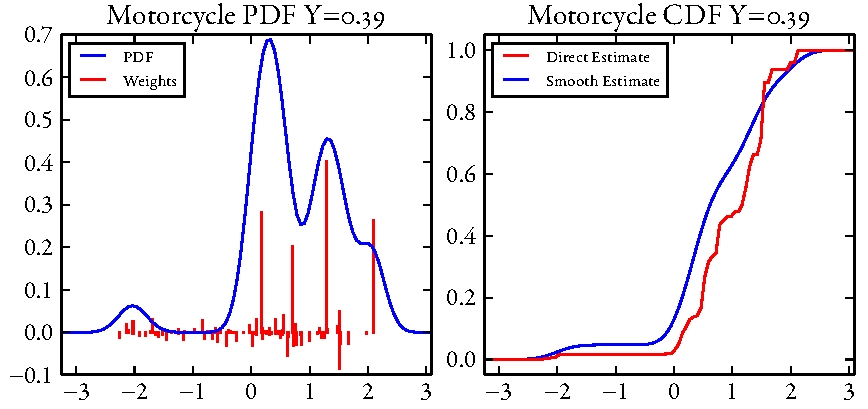
\includegraphics[width=\columnwidth]{figures/cumulativeexamplesmooth}
				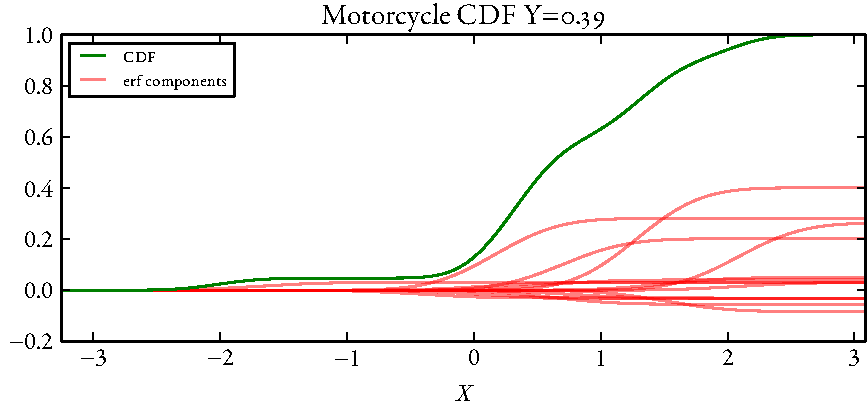
\includegraphics[width=\columnwidth]{figures/cumulativeexampleerf}
			\end{center}
			\caption{\small (Left) The PDF obtained through the pre-image method on the Motorcycle dataset (blue) and The embedding weights at the training points (red). (Right) The resulting CDF estimate using the direct estimate \eqref{eq:empirical_cdf} and smooth estimate \eqref{eq:smooth_empirical_cdf_gaussian_kernel}. (Bottom) The smooth CDF estimate again (green) with its individual error function components (red) overlayed \eqref{eq:qpi_empirical_cdf_gaussian_kernel}.}
			\label{fig:discriminative_quantile_regression}
		\end{figure}
		
		By embedding indicator functions, the resulting CDF estimate \eqref{eq:empirical_cdf} is discontinuous at the jumps located at each data point. Directly differentiating this would result in a superposition of Dirac deltas for the PDF. However, in many applications, the PDF is rather smooth, and thus so is the CDF. Many characteristic kernels are also smooth, and thus so are the functions within their RKHS. Therefore, instead of taking the inner product between the embedding and the indicator function, we propose to take the inner product with a function $\tilde{\mathbb{1}}_{A}$ \eqref{eq:indicator_smooth} that is within the full RKHS $\mathcal{H}_{k}$ and converges to the indicator function $\mathbb{1}_{A}$ as the kernel bandwidth goes to zero.
		
		\begin{equation}
			\tilde{\mathbb{1}}_{A} := \int_{A} k(\bvec{x}, \cdot) d\bvec{x} = \int_{A} \phi_{\bvec{x}} d\bvec{x}
		\label{eq:indicator_smooth}
		\end{equation}
		
		This results in a distribution estimate \eqref{eq:smooth_empirical_distribution} and CDF estimate \eqref{eq:smooth_empirical_cdf} that are smooth.

		\begin{equation}
		\begin{aligned}
			\hat{\mathbb{P}}_{\bvec{\rv{X}}}[A] &= \langle \hat{\mu}_{\bvec{\rv{X}}}, \tilde{\mathbb{1}}_{A} \rangle = \hat{\mu}_{\bvec{\rv{X}}}^{T} \tilde{\mathbb{1}}_{A} = (\Phi_{\ds{X}} \bm{\beta})^{T} \int_{A} \phi_{\bvec{x}} d\bvec{x} \\
			&= \bm{\beta}^{T} \Phi_{\ds{X}}^{T} \int_{A} \phi_{\bvec{x}} d\bvec{x} = \int_{A} \bm{\beta}^{T} \Phi_{\ds{X}}^{T} \phi_{\bvec{x}} d\bvec{x} \\
			&= \int_{A} \bm{\beta}^{T} K_{\ds{X} \bvec{x}} d\bvec{x} = \int_{A} \sum_{i = 1}^{n} \beta_{i} k(\bvec{x}_{i}, \bvec{x}) d\bvec{x} \\
			&= \sum_{i = 1}^{n} \beta_{i} \int_{A}  k(\bvec{x}_{i}, \bvec{x}) d\bvec{x} \\
		\end{aligned}
		\label{eq:smooth_empirical_distribution}
		\end{equation}	
		
		\begin{equation}
			\hat{P}_{\bvec{\rv{X}}}(\bvec{x}) := \hat{\mathbb{P}}_{\bvec{\rv{X}}}[(-\bvec{\infty}, \bvec{x}]] = \sum_{i = 1}^{n} \beta_{i} \int_{(-\bvec{\infty}, \bvec{x}]}  k(\bvec{x}_{i}, \bvec{x}') d\bvec{x}'
		\label{eq:smooth_empirical_cdf}
		\end{equation}
		
		The estimates are expressed as a summation of the kernel integrals, which would need to be analytically derived or otherwise estimated. For a Gaussian kernel, analytical form can be derived \eqref{eq:smooth_empirical_cdf_gaussian_kernel}. Even if analytical form cannot be derived for some kernels $k$, since it is independent of the embedding weights, the integral $\bvec{k}_{\ds{X}}$ \eqref{eq:kernel_integral} can be approximated and pre-computed before inference begins.

		\begin{equation}
			\hat{P}_{\bvec{\rv{X}}}(\bvec{x}) = \frac{1}{2} \sum_{i = 1}^{n} \beta_{i} \prod_{j = 1}^{d} \Bigg[1 + \mathrm{erf}\bigg(\frac{x_{j} - x_{i, j}}{\sigma_{j} \sqrt{2}}\bigg)\Bigg]
		\label{eq:smooth_empirical_cdf_gaussian_kernel}
		\end{equation}

		\begin{equation}
			\hat{P}_{\bvec{\rv{X}}}(\bvec{x}) = \bm{\beta}^{T} \bvec{k}_{\ds{X}} \; : \; \bvec{k}_{\ds{X}} := \Bigg\{ \int_{(-\bvec{\infty}, \bvec{x}]}  k(\bvec{x}_{i}, \bvec{x}') d\bvec{x}' \Bigg\}_{i = 1}^{n}
		\label{eq:kernel_integral}
		\end{equation}
			
		With this approach, CDF estimates are now smooth and can be shown to converge to the true CDF in the limit of $n \rightarrow \infty$ and vanishing kernel bandwidth. However, due to the possibility of negative weights $\beta_{i}$, both discriminative approaches may produce CDF estimates that are not strictly non-decreasing, as shown in \cref{fig:discriminative_quantile_regression}. Notice that the direct non-smooth direct CDF estimate jumps at locations corresponding to training points, and that, due to the negative weights, the smooth CDF estimate contain components that go below zero such that the resultant CDF estimate may not be strictly non-decreasing. Furthermore, the resulting CDF may not be in the range $[0, 1]$. To rectify this, we propose a generative approach to estimating the CDF.

\section{Generative Quantile Regression}
\label{sec:generative_quantile_regression}

%	\warn{So we need to cite MKBR before we talk about integrating it. The integration part is relatively short and straight forward, so the section would comprise of deriving and discussing MKBR with examples, and then discuss integration briefly, and then present example figures.}
	
	Given a particular embedding, the empirical PDF can be recovered through the quadratic programming pre-image (\qpi) method proposed by \cite{McCalman2013}. This method represents the PDF as a mixture of the kernel $k$ centred at each of the data points, and thus has as many components as the number of data points. Through minimising the RKHS distance between the true PDF and the PDF estimate, the resulting algorithm reduces to a tractable quadratic programming optimisation problem, which finds the optimal weights $\{w_{i}\}_{i = 1}^{n}$ for which $\hat{p}_{\bvec{\rv{X}}}$ is closest to the true PDF \eqref{eq:qpi}. 
	
	\begin{equation}
		\hat{p}_{\bvec{\rv{X}}}(\bvec{x}) = \sum_{i = 1}^{n} w_{i} k(\bvec{x}_{i}, \bvec{x})
	\label{eq:qpi}
	\end{equation}

	Since \qpi recovers a valid PDF that is as smooth as the kernel $k$, integrating this PDF would result a smooth, proper distribution $\hat{\mathbb{P}}_{\bvec{\rv{X}}}$ \eqref{eq:qpi_empirical_distribution} and CDF $\hat{P}_{\bvec{\rv{X}}}$ \eqref{eq:qpi_empirical_cdf} that is always non-decreasing.
	
	\begin{equation}
		\hat{\mathbb{P}}_{\bvec{\rv{X}}}[A] = \int_{A} \hat{p}_{\bvec{\rv{X}}}(\bvec{x}) d\bvec{x} = \sum_{i = 1}^{n} w_{i} \int_{A} k(\bvec{x}_{i}, \bvec{x}) d\bvec{x}
	\label{eq:qpi_empirical_distribution}
	\end{equation}
	
	\begin{equation}
		\hat{P}_{\bvec{\rv{X}}}(\bvec{x}) := \hat{\mathbb{P}}_{\bvec{\rv{X}}}[(-\bvec{\infty}, \bvec{x}]] = \sum_{i = 1}^{n} w_{i} \int_{(-\bvec{\infty}, \bvec{x}]} k(\bvec{x}_{i}, \bvec{x}') d\bvec{x}'
	\label{eq:qpi_empirical_cdf}
	\end{equation}
	
	Similar to the smooth distribution estimate \eqref{eq:smooth_empirical_distribution} and CDF estimate \eqref{eq:smooth_empirical_cdf}, the estimates \eqref{eq:qpi_empirical_distribution} and \eqref{eq:qpi_empirical_cdf} require the integral of the kernel $k$, which can either be analytically derived or at least approximated and pre-computed beforehand. Again, analytical form is available for Gaussian kernels \eqref{eq:qpi_empirical_cdf_gaussian_kernel}.
	
	\begin{equation}
		\hat{P}_{\bvec{\rv{X}}}(\bvec{x}) = \frac{1}{2} \sum_{i = 1}^{n} w_{i} \prod_{j = 1}^{d} \Bigg[1 + \mathrm{erf}\bigg(\frac{x_{j} - x_{i, j}}{\sigma_{j} \sqrt{2}}\bigg)\Bigg]
	\label{eq:qpi_empirical_cdf_gaussian_kernel}
	\end{equation}
	
	This CDF estimate is essentially of the same form as the smooth discriminative estimate \eqref{eq:smooth_empirical_cdf_gaussian_kernel}, but with the embedding weights $\bm{\beta}$ replaced by the recovered density weights $\bvec{w}$. Since the density weights $\bvec{w}$ are by construction of \qpi always positive, unlike the embedding weights $\bm{\beta}$, the resulting CDF is guaranteed to be non-decreasing. This form equivalence also highlights the fact that the smooth CDF estimate is simply the integral of the normalised embedding.
		
\section{Hyperparameter Learning}
\label{sec:hyperparameter_learning}

	With all kernel based techniques, the kernel $k = k_{\bm{\theta}}$ itself is usually specified from a family of kernels parametrised by some hyperparameters $\bm{\theta}$. For example, a Gaussian kernel would be specified by its length scale parameters. The number of parameters would depend on whether the kernel is isotropic ($1$ parameter), anisotropic axis-aligned ($d$ parameters), or general ($d(d - 1)/2$ parameters). Whichever family we choose, we would have to find the optimal hyperparameter setting that gives the best performance in terms of inference accuracy.
	
	We considered two approaches to hyperparameter learning for the purpose of quantile regression.
	
%	\begin{equation}
%		L_{\rv{X}, \tau}(x) = \left\{ \begin{array}{lr}
%			(x - q_{\rv{X}}(\tau)) \tau & : x \geq q_{\rv{X}}(\tau) \\
%			(q_{\rv{X}}(\tau) - x) (1 - \tau) & : x <  q_{\rv{X}}(\tau)
%		\end{array} \right.
%	\end{equation}
	
	The first approach involves minimising the expected pinball loss \eqref{eq:expected_pinball_loss} for a given dataset $\ds{X} := \{x_{i}\}_{i = 1}^{n}$, where the pinball loss is defined by \eqref{eq:pinball_loss}. The minimiser of the expected pinball loss \eqref{eq:expected_pinball_loss} is the $\tau$-quantile $z = q_{\rv{X}}(\tau)$ of the distribution $\mathbb{P}_{\rv{X}}$ \citep{Koenker1978}.
	
	\begin{equation}
		L_{\tau}(x, z) = \left\{ \begin{array}{lr}
			(x - z) \tau & : x \geq z \\
			(z - x) (1 - \tau) & : x < z
		\end{array} \right.
	\label{eq:pinball_loss}
	\end{equation}
	
	This expected pinball loss \eqref{eq:expected_pinball_loss} to be minimised is evaluated over a leave-out validation set from the available training data obtained from a standard cross-validation procedure. We will call this approach \textit{pinball learning}.
	
	\begin{equation}
		\bar{L}_{\tau}(\ds{X}, z) := \frac{1}{n} \sum_{i = 1}^{n} L_{\tau}(x_{i}, z)
	\label{eq:expected_pinball_loss}
	\end{equation}
	
	For a particular quantile, a function which minimises the pinball loss will also minimise the
	error in the quantile estimate. Additionally, this loss function is tolerant to CDF estimates which may not be strictly non-decreasing, such as \eqref{eq:empirical_cdf} and \eqref{eq:smooth_empirical_cdf}. This however also means that the loss function is specific to a particular quantile such that each quantiles estimate requires separate optimisations despite using the same training set. The result is that quantile estimates may actually cross for certain query locations, a phenomenon known as quantile crossing.
	
	Another possible approach to parameter learning is to optimise the parameters with respect to the joint probability of observing the collected dataset \eqref{eq:lml}, also called the evidence. Evaluated over the whole training set, this is akin to method of log marginal likelihood optimisation in the Gaussian process context. However, here we again choose to only evaluate it over a leave-out validation set. We will call this approach \textit{evidence learning}. The advantage of this approach is that it is independent of the particular quantile estimate chosen. As such, a single, consistent CDF is generated for all quantile queries, eliminating the possibility of quantile crossing. 
	
	\begin{equation}
		p_{\rv{X}^{(n)}, \bm{\theta}}(x_{1}, \cdots, x_{n}) = \sum_{i = 1}^{n} \log(\hat{p}_{\rv{X}, \bm{\theta}}(x_{i}))
	\label{eq:lml}
	\end{equation}
	
	However, clearly this requires the PDF to be estimated first, even though discriminative approaches do not require them. Thus, this method is more natural in the generative approach. Nevertheless, this is only required during the learning stage. Once the optimal hyperparameters are obtained, one can choose to use the resulting hyperparameters in the discriminative approach for inference.
	
\section{Quantile Regression Algorithms}
\label{sec:quantile_regression_algorithms}
	
	Suppose some data $\{(\bvec{y}_{i}, x_{i})\}_{i = 1}^{n}$ is collected from a joint distribution $\mathbb{P}_{\rv{Y} \rv{X}}$. We can either find the standard empirical embedding $\hat{\mu}_{\rv{X}}$ or empirical conditional embedding $\hat{\mu}_{\rv{X} | \bvec{\rv{Y}} = \bvec{y}}$, both of which is of the form $\Phi_{\ds{X}} \bm{\beta}$ for some weights. This is also true for posterior embeddings obtained from KBR. In this paper we present four main methods for quantile regression. 	Table \ref{table:quantile_regression_methods} lists the properties of each of these algorithms.

	\theoremstyle{definition}
	\begin{definition}
		(Direct Embedding Quantile Estimator)
		The direct embedding $\tau$-quantile estimate is
		\begin{equation}
			q_{\rv{X}}(\tau) = \min\{x \in \mathbb{R} : \frac{1}{\Vert \bm{\beta} \Vert} \sum_{i : x_{i} \leq x} \beta_{i} \geq \tau\}
		\end{equation}	
		The hyperparameter learning is done by minimising the pinball loss \eqref{eq:expected_pinball_loss} of the training data using cross-validation. We denote this algorithm as DR.
	\end{definition}
	
	\theoremstyle{definition}
	\begin{definition}
		(Smooth Embedding Quantile Estimator)
		The smooth embedding $\tau$-quantile estimate is
		\begin{equation}
			q_{\rv{X}}(\tau) = x : \frac{1}{\Vert \bm{\beta} \Vert} \bm{\beta}^{T} \bvec{k}_{\ds{X}} = \tau
		\end{equation}	
		The hyperparameter learning is done by minimising the pinball loss \eqref{eq:expected_pinball_loss} of the training data using cross-validation. We denote this algorithm as DS.
	\end{definition}
	
	\theoremstyle{definition}
	\begin{definition}
		(Pre-Image Quantile Estimator)
		The pre-image $\tau$-quantile estimate is
		\begin{equation}
			q_{\rv{X}}(\tau) = x : \bvec{w}^{T} \bvec{k}_{\ds{X}} = \tau
		\end{equation}	
		where $\bvec{w}$ is are the recovered density weights from QPI.
		Both pinball learning and evidence learning can be used. We denote this algorithm as JB with done with pinball learning, and JL when done with evidence learning.
	\end{definition}
	
	\theoremstyle{definition}
	\begin{definition}
		(Normed Weights Quantile Estimator)
		The pre-image $\tau$-quantile estimate is
		\begin{equation}
		q_{\rv{X}}(\tau) = x : \bvec{\tilde{w}}^{T} \bvec{k}_{\ds{X}} = \tau
		\end{equation}
		where $\bvec{\tilde{w}}$ is the clip-normalised weights of the relevant embedding.
		Both pinball learning and evidence learning can be used. We denote this algorithm as NB with done with pinball learning, and NL when done with evidence learning.
	\end{definition}	
	
	\begin{table}[t!]
		\begin{center}
			\begin{tabular}{l|cccc}
				Algorithm & S & ND &   NC & Complexity \\ \hline
				DR  &              &                &                & $O(n \log(n))$    \\
				DS  & $\checkmark$ &                &                &
				$O(n \log(n))$  \\
				NB  & $\checkmark$ & $\checkmark$   &                &
				$O(n \log(n))$ \\
				JB  & $\checkmark$ & $\checkmark$   &                &
				$O(n^{3} \log(n))$ \\
				NL  & $\checkmark$ & $\checkmark$   & $\checkmark$   &
				$O(n \log(n))$ \\
				JL  & $\checkmark$ & $\checkmark$   & $\checkmark$   &   $O(n^{3} \log(n))$ 
			\end{tabular}
		\end{center}
		\caption{Comparison of Quantile estimation techniques. S stands for Smooth, ND for Non-Decreasing, and NC for Non-Crossing. For complexity, $n$ is the number of training points.}
		\label{table:quantile_regression_methods}
	\end{table}
	
%	\subsection{Computational Complexity}
%	\label{sec:quantile_regression_algorithms:computational_complexity}
		
	The computational complexity of these algorithms varies from $O(n \log(n))$ to $O(n^{3} \log(n))$ in the number of training points $n$. The 1-D root-finding required to solve the quantile equations adds a factor of $\log(n)$ in all cases (using a binary search), the difference comes from the cumulative estimation algorithms.
	
	The cheapest cumulative evaluate is the direct embedding estimator (DR) --- this is simply a (conditional) sum of the mixture weights and is therefore $O(n)$ in the number of training points. The smooth embedding estimator (DS) and the normed weights estimator (NL and NB) are also inexpensive to compute, provided an efficient estimate of the kernel integral exists. They are also $O(n)$, but with a larger constant due to the kernel integration. The most expensive are the pre-image estimators (JL and JB), which require solving a quadratic program to determine the mixture weights and are therefore $O(n^3)$. This is only relevant if a PDF estimate was not required, and the pre-image was computed only for the quantiles. If a pre-image estimate is already available then the JL and JB are also $O(n)$.
	
\section{Related Work}
\label{sec:related_work}

	Quantile regression was first introduced by \cite{Koenker1978}. This work considered the regression problem of inferring values of an unknown linea model given noisy samples of inputs and outputs. Rather than using the mean as an estimator of the function, Koenker chose the 0.5 quantile (the median), on the basis that it was less sensitive to outliers, and hence effective in cases with non-Gaussian or heavy tailed noise. A general regression quantile was then defined as the function value minimising the pinball loss \citep{Koenker1978}. For linear models, the minimisation was formulated as a linear programming problem and so solved efficiently.
	
	The pursuit of conditional quantiles quickly divided the field into so-called discriminative methods, that attempt to directly compute the quantile from the training data through minimisation of the pinball loss, and generative methods, that attempt to first model the conditional cumulative distribution, and from there derive quantile estimates \citep{Koenker2005}.
	
	The discriminative initially demonstrated the advantage of flexibility --- non-parametric function estimation techniques could be applied that made no assumptions about the underlying distribution. Examples include locally-constant and locally-linear approximations \citep{Chaudhuri1991, Yu1998}. However, this flexibility also led to problems such as quantile crossing; in which a data point might be considered to be below the 0.5 quantile but above the 0.6 quantile\cite{Koenker2005}. 
	
	An important development was the addition of non-crossing constraints to discriminative quantile regression solutions \citep{He1997}. This ensured that different quantile estimates obeyed a strict ordering, with no two quantiles having the same function value. Such a strict ordering was achieved by adding a penalty term to the optimisation \citep{Cole1992}, or by reducing the class of possible functions used to represent the quantiles, for instance to classes of location-scale models \citep{Koenker1984, He1997}. Unfortunately, such models implicitly restricted the underlying distribution, causing reduced applicability to data that did not fit the assumptions of the model \citep{Koenker2005}.
	
	Standard machine learning techniques have also been co-opted for conditional quantile estimation, including the support vector machine (SVM), which finds the decision boundary associated with the minimisation of the pinball loss, with additional non-crossing constraints \citep{Takeuchi2006}. However, in this algorithm, the non-crossing constraints may cause the resulting estimates to violate the (empirical) quantile definition.
	
	More recently, Chernozhukov et. al. developed a monotisation procedure based on function re-arrangement to remove crossing from quantile estimates generated by other algorithms. The resulting quantiles were guaranteed to be more accurate, and no assumptions were made about the underlying distribution \citep{Chernozhukov2010}.
	
	The `quanting' algorithm \citep{Langford2006} introduced an important development in discriminative estimation of conditional quantiles, which was to re-cast quantile regression as a classification problem. By placing a set of classifiers over the range of the regression, each classifier can be trained on whether the quantile is above or below it. The quantile estimate is then the expectation of this assignment, over all the classifiers.  A set of importance weights were learned to minimise the error of the estimation.
	
	Generative models for conditional quantile regression have also been examined in the semi-parametric and non-parametric setting. Linear models for Bayesian quantile estimation were examined in \cite{Yu2001}, using Laplacian likelihood functions and uniform priors. These methods require Markov chain Monte Carlo (MCMC) integration to perform inference, as well as making the uni-modal assumption. Similar semi-parametric methods such as \cite{Hjort2006, Hjort2009} use Dirichlet process priors, which again required costly inference approximations.
	
	Kernel conditional quantiles using Gaussian process regression to explicitly compute the cumulative distribution were examined by \cite{Quadrianto2009}. The underlying PDF was estimated using a Gaussian process, which enforced the non-crossing constraint and allowed for efficient inference. Additionally, heteroskedastic covariance functions were employed to account for input-dependent noise in the data. One limitation of the work was that the underlying Gaussianity assumption restricts applicability to uni-modal distributions.
	
	A more general formulation of Bayesian quantile regression was developed in \cite{Taddy2010}, which used Dirichlet process mixture models to represent the underlying joint distribution. This allowed a very general class of distributions to be represented, but inference required expensive MCMC integration.
	
	% Indicator co-Kriging in a non-parametric approach in the geo-statistics
	% literature based on explicit modelling of the underlying distribution through
	% Kriging~\cite{Pardo2005}.
	
	% check chen and muller 2012 for a nonparametric CDF
	% approach~\cite{Chen2012} 
	
	Our work aims to overcome limitations of both these methods-- giving the flexibility of a mixture distribution representation for modelling multi-modal behaviour, with the efficient inference inherent in the pre-image algorithm. It is to this new algorithm we now turn our attention.

\section{Experiments}
\label{sec:experiments}

	We now test the performance of our quantile estimators on a number of standard machine learning datasets. We compare our algorithms to state-of-the-art generative and discriminative techniques for conditional quantile estimation.
	
	We evaluated the algorithms on four datasets commonly used in the literature for conditional quantile estimation tests: Antigen, Weather, Bone Mineral Density, and Motorcycle. The Antigen dataset samples the concentration of various molecules \citep{Quadrianto2009} in a blood sample. The dataset contains 97 points, with eight-dimensional observations $\bvec{y}$ and a one-dimensional state $x$. The Weather dataset measures a meteorological variable distributed over the surface of the Earth. It has two-dimensional observations $\bvec{y}$ and a one-dimensional state $\bvec{x}$, and contains 238 points. The Motorcycle dataset is a record of measurements taken from an accelerometer during a front-on motorcycle collision, and is often used because it contains heteroskedastic, non-Gaussian behaviour. The dataset contains 137 points, with a single input dimension $y$ (time), and a single output dimension $x$. Finally, the Bone Mineral Density dataset contains relative spinal bone mineral density measurements from North American adolescents of various ages. It has a single input variable $y$ (age), a single output variable $x$ (bone mineral density), and 485 points. The original data were recorded by \cite{Bachrach1999}. Antigen, Weather and Motorcycle were taken from the UCI repository \citep{Bache2013} and Bone Mass Density from the ``ElemStatLearn'' R package \citep{Hastie2005}.
	
	For all experiments, performance was evaluated by five-fold cross validation and the average pinball loss over the hold-out set. The average and standard deviation of the performance over these five tests was used as the final score. Three quantiles were tested for each dataset; 0.1, 0.5 and 0.9. Any categorical variables in the data were ignored. All input and output variables were scaled to have zero mean and unit variance in each dimension.
	
	We place a Gaussian kernel for both the input variable $y$ and the output variable $x$. For the input variable $y$, we whiten the data to decorrelate each dimension using a form of automatic relevance determination \citep{Rasmussen2006} such that an anisotropic but diagonal Gaussian kernel can be used. All our algorithms were trained with (nested) five-fold cross-validation.
	
	\subsection{Comparisons}
	\label{sec:experiments:comparison}
	
		Below we summarise the algorithms we are comparing our algorithms with \cite{Quadrianto2009}.
		
		\textbf{Linear Quantile Estimation}. (Algorithm A) This is the linear discriminative	quantile estimator described in \cite{Koenker1978}.
		
		\textbf{Quantile SVM}. (Algorithm B) This is a non-parametric quantile estimator based on dual optimisation of the loss function through a SVM, as documented in \cite{Takeuchi2006}. A RBF kernel was used for this algorithm, with kernel width and regularisation fitted as described in \cite{Quadrianto2009}.

		\textbf{Reduction to Classification}. (Algorithm C) This is the algorithm for reducing a quantile estimation problem to a series of classifiers \citep{Langford2006}. The results from this algorithm are taken from \cite{Quadrianto2009}, which used 100 GP classifiers trained with expectation propagation and an RBF kernel.
		
		\textbf{Quantile GP}. (Algorithm D) (Algorithm D) This algorithm is the Gaussian-processed based direct CDF estimate \cite{Quadrianto2009}. An RBF kernel was used, with the hyper-parameters learned by optimising the marginal log-likelihood.
		
		\textbf{Heteroskedastic Quantile GP}. (Algorithm E) This algorithm is the same as the Quantile GP, except that the kernel is a heteroskedastic RBF with 10 latent pseudo-observations controlling the bandwidth along the length of the input dimension \citep{Quadrianto2009}. 
		
	\subsection{Results}
	\label{sec:experiments:results}
	
		\begin{figure*}[!htbp]
			\centering
			\begin{subfigure}[b]{0.32\textwidth}
				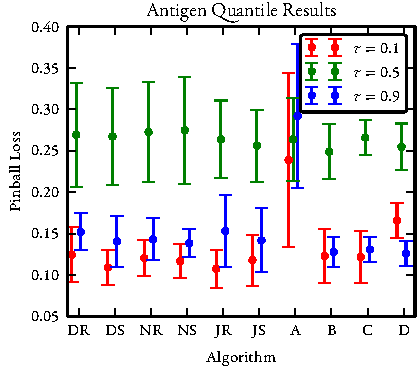
\includegraphics[width=\textwidth]{figures/Antigen_results}
			\end{subfigure}
			\begin{subfigure}[b]{0.32\textwidth}
				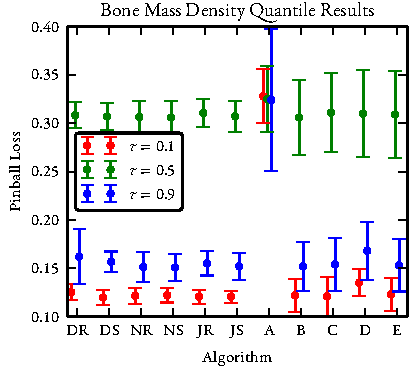
\includegraphics[width=\textwidth]{figures/Bone_Mass_Density_results}
			\end{subfigure}
			\begin{subfigure}[b]{0.32\textwidth}
				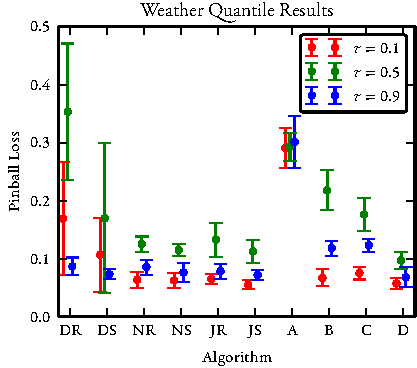
\includegraphics[width=\textwidth]{figures/Weather_results}
			\end{subfigure}
			\caption{Results from the three quantile experiments. The error bars in these
				figures represent $\pm 1$ standard deviation of the pinball loss over the testing set.}
			\label{fig:qfull}
		\end{figure*}

		\begin{figure}[!htbp]
			\begin{center}
				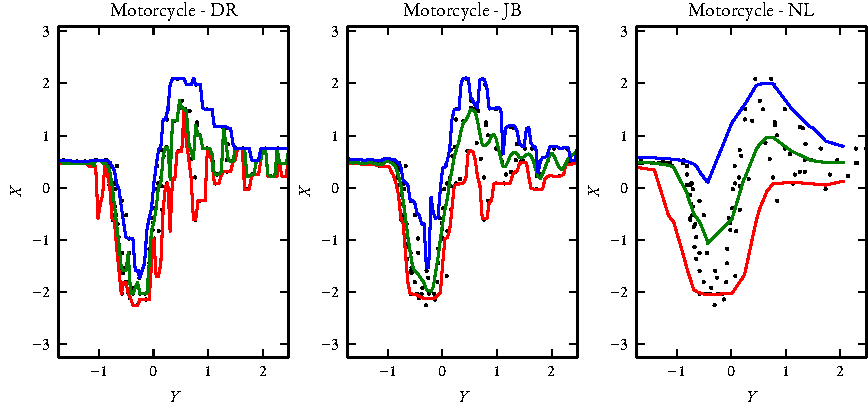
\includegraphics[width=\columnwidth]{figures/mcquantilesall}\\
			\end{center}
			\caption{Examples of 0.1 (red), 0.5 (green) and 0.9 (blue) quantile estimates
				for the Motorcycle dataset, for the DR (left), JB (centre) and NL (right) algorithms.}
			\label{fig:motorcycleresults} 
		\end{figure}
		
		\begin{table}
			\begin{center}
				\begin{tabular}{l|ccc}
					Alg. & $\tau = 0.1$     & $\tau = 0.5$  & $\tau = 0.9$      \\ \hline
					DR & $0.125 \pm 0.033$ & $0.270 \pm 0.063$ & $0.152 \pm 0.022$ \\
					DS & $\mathbf{0.109 \pm 0.022}$ & $0.267 \pm 0.059$ & $0.141 \pm 0.031$ \\
					NB & $0.117 \pm 0.021$ & $0.275 \pm 0.065$ & $0.139 \pm 0.017$ \\
					JB & $0.118 \pm 0.031$ & $0.256 \pm 0.044$ & $0.142 \pm 0.039$ \\
					NL & $0.136 \pm 0.035$ & $0.294 \pm 0.030$ & $0.141 \pm 0.014$ \\
					JL & $0.124 \pm 0.017$ & $0.260 \pm 0.033$ & $0.132 \pm 0.022$ \\
					A & $0.239 \pm 0.105$ & $0.264 \pm 0.050$ & $0.292 \pm 0.087$ \\
					B & $0.123 \pm 0.033$ & $\mathbf{0.249 \pm 0.033}$ & $0.128 \pm 0.018$ \\
					C & $0.122 \pm 0.031$ & $0.266 \pm 0.021$ & $0.131 \pm 0.015$ \\
					D & $0.166 \pm 0.021$ & $0.255 \pm 0.028$ & $\mathbf{0.126 \pm 0.015}$
				\end{tabular}
			\end{center}
			\caption{Antigen results.}
			\label{table:antigen}
		\end{table}
		
		\begin{table}
			\begin{center}
				\begin{tabular}{l|ccc}
					Alg. & $\tau = 0.1$     & $\tau = 0.5$  & $\tau = 0.9$      \\ \hline
					DR & $0.169 \pm 0.098$ & $0.353 \pm 0.117$ & $0.086 \pm 0.015$ \\
					DS & $0.106 \pm 0.064$ & $0.169 \pm 0.129$ & $0.073 \pm 0.009$ \\
					NB & $\mathbf{0.062 \pm 0.012}$ & $0.115 \pm 0.010$ & $0.076 \pm 0.016$ \\
					JB & $0.055 \pm 0.008$ & $0.112 \pm 0.020$ & $0.072 \pm 0.009$ \\
					NL & $0.063 \pm 0.008$ & $0.143 \pm 0.029$ & $0.087 \pm 0.016$ \\
					JL & $0.077 \pm 0.012$ & $0.136 \pm 0.034$ & $0.094 \pm 0.016$ \\
					A & $0.291 \pm 0.034$ & $0.293 \pm 0.024$ & $0.301 \pm 0.045$ \\
					B & $0.067 \pm 0.015$ & $0.218 \pm 0.034$ & $0.118 \pm 0.013$ \\
					C & $0.075 \pm 0.011$ & $0.176 \pm 0.028$ & $0.123 \pm 0.011$ \\
					D & $0.057 \pm 0.010$ & $\mathbf{0.097 \pm 0.015}$ & $\mathbf{0.068 \pm 0.017}$
				\end{tabular}
			\end{center}
			\caption{Weather results.}
			\label{table:weather}
		\end{table}
		
		
		\begin{table}
			\begin{center}
				\begin{tabular}{l|ccc}
					Alg. & $\tau = 0.1$     & $\tau = 0.5$  & $\tau = 0.9$      \\ \hline
					DR & $0.163 \pm 0.060$ & $0.240 \pm 0.037$ & $0.096 \pm 0.024$ \\
					DS & $0.180 \pm 0.075$ & $0.465 \pm 0.181$ & $0.120 \pm 0.022$ \\
					NB & $0.096 \pm 0.019$ & $0.194 \pm 0.033$ & $0.092 \pm 0.015$ \\
					JB & $0.101 \pm 0.030$ & $0.204 \pm 0.022$ & $0.107 \pm 0.041$ \\
					NL & $0.097 \pm 0.016$ & $0.210 \pm 0.034$ & $0.092 \pm 0.016$ \\
					JL & $0.091 \pm 0.007$ & $0.199 \pm 0.032$ & $0.091 \pm 0.010$ \\
					A & $0.396 \pm 0.080$ & $0.389 \pm 0.019$ & $0.387 \pm 0.056$ \\
					B & $0.090 \pm 0.012$ & $0.202 \pm 0.019$ & $0.085 \pm 0.008$ \\
					C & $0.094 \pm 0.011$ & $0.190 \pm 0.015$ & $0.083 \pm 0.010$ \\
					D & $0.092 \pm 0.025$ & $\mathbf{0.186 \pm 0.018}$ & $0.089 \pm 0.010$ \\
					E & $\mathbf{0.079 \pm 0.019}$ & $0.187 \pm 0.021$ & $\mathbf{0.070 \pm
						0.016}$
				\end{tabular}
			\end{center}
			\caption{Motorcycle results.}
			\label{table:motorcycle}
		\end{table}
		
		
		\begin{table}
			\begin{center}
				\begin{tabular}{l|ccc}
					Alg. & $\tau = 0.1$     & $\tau = 0.5$  & $\tau = 0.9$      \\ \hline
					DR & $0.125 \pm 0.008$ & $0.308 \pm 0.013$ & $0.162 \pm 0.028$ \\
					DS & $\mathbf{0.120 \pm 0.007}$ & $0.307 \pm 0.014$ & $0.157 \pm 0.011$ \\
					NB & $0.122 \pm 0.007$ & $\mathbf{0.306 \pm 0.017}$ & $\mathbf{0.151 \pm
						0.014}$ \\
					JB & $0.121 \pm 0.006$ & $0.307 \pm 0.016$ & $0.152 \pm 0.014$ \\
					NL & $0.121 \pm 0.016$ & $0.308 \pm 0.013$ & $0.153 \pm 0.011$ \\
					JL & $0.123 \pm 0.014$ & $\mathbf{0.306 \pm 0.012}$ & $0.153 \pm 0.013$ \\
					A & $0.328 \pm 0.028$ & $0.325 \pm 0.034$ & $0.324 \pm 0.073$ \\
					B & $0.122 \pm 0.017$ & $\mathbf{0.306 \pm 0.039}$ & $0.152 \pm 0.025$ \\
					C & $0.121 \pm 0.020$ & $0.311 \pm 0.041$ & $0.154 \pm 0.027$ \\
					D & $0.135 \pm 0.014$ & $0.310 \pm 0.045$ & $0.168 \pm 0.030$ \\
					E & $0.123 \pm 0.017$ & $0.309 \pm 0.045$ & $0.153 \pm 0.027$
				\end{tabular}
			\end{center}
			\caption{Bone Mineral Density results.}
			\label{table:bmd}
		\end{table}
		
		The average pinball loss for each algorithm in the three experiments is given in \cref{fig:qfull}. Overall, generative algorithms performed as well if not better than the algorithms from the literature. The two best performing algorithms were NB and JB, which are the normed-weights and \qpi methods, trained under the pinball loss. It is unsurprising that pinball learning performed better than evidence learning, given that the training was optimising the same function that would evaluate the algorithm's performance.

		This demonstrates a trade-off between using pinball loss and receiving slightly better performance, or using negative log evidence probability (NL and JL) and ensuring the non-crossing constraint holds. The NL and JL algorithms were still competitive, but also beaten out by the kernel conditional quantile (D).

		With both the pinball learning and evidence learning, there was little difference on average between the pre-image estimator and the normed-weights estimator. This fact in particular is worth noting when considering a real-time application of these algorithms, as the pre-image estimator has a much greater computational cost.
		
		Over the three experiments, we see that extremal quantiles 0.1 and 0.9 have significantly lower pinball loss compared to the median (0.5). There appear to be no algorithm that is especially capable at a particular quantile, although two direct methods (DR and DS) are much more competitive with the extrema than the median. The likely explanation is that, in general, an accurate (empirical) estimate of the median is affected by nearby points both above and below it. These direct methods however only sum contributions from points lying below the median. The pre-image methods on the other hand, sum contributions from mixture components centred at all training points. Far away from the median, there are fewer points nearby and so the effect is reduced.
		
		The full results for each individual experiment and quantile are also tabulated. For Antigen, this information is given in \cref{table:antigen}. Curiously, the three top performers for the quantiles were each from a totally different family of algorithms. Our smooth direct embedding estimator (DS), the quantile SVM (B), and the quantile GP (D). The full results for the Weather, and Bone Mineral Density tests are given in \cref{table:weather} and \cref{table:bmd}.
		
		From \cref{table:motorcycle} and \cref{table:bmd}, we can see that algorithm E matched or exceeded all other algorithms in Motorcycle dataset, and was competitive but did not beat our algorithms in the Bone Mineral Density dataset. The likely explanation is the strong heteroskedasicity of the Motorcycle dataset benefited from a modelling approach that explicitly took it into account. This raises a possible avenue of future work--- including heteroskedastic kernel in our methods to improve performance.
		
		Figure \ref{fig:motorcycleresults} plots the quantiles estimated for the Motorcycle dataset for three of the algorithms. The piecewise-constant quantile estimates are clearly visible in the DR plot. The JB plot has each quantile trained separately, and as a result the 0.1 and 0.9 quantile both fit the boundary of the data very closely. The NL plot shows a much smoother representation, in line with the fact that these are quantiles for a single underlying cumulative distribution (trained with the negative log evidence probability).

\section{Conclusion}
\label{sec:conclusion}

	\warn{Future work would include a better learning method for the hyperparameters, and also a better density recovery method for the generative approach besides \qpi.}
	
	This paper presented six new algorithms for estimating quantiles non-parametrically from kernel embeddings of probability distributions given only samples. By projecting the indicator function into the RKHS, we first present a discriminative approach where the empirical CDF can be computed directly, but lack the the desired smoothness and non-decreasing property. We then impose smoothness by instead projecting a smooth function within the full RKHS that becomes the projected indicator function in the limit of vanishing bandwidth. At a trade off with computational complexity, the non-decreasing constraint is guaranteed by a generative approach, where the embeddings weights of a PDF is to be recovered from a quadratic program first, before it is integrated to a CDF.
	
	We then constructed quantile estimators from these CDF estimators using simple numerical root-finding, and considered training on both the pinball loss function, and the negative log evidence probability. We then evaluated the resulting algorithms using a set of well-known machine learning datasets.
	
	Our generative quantile estimators in particular were comparable to, or better than, the state-of-the-art algorithms in the literature. These algorithms can be trained either using pinball loss, for a slight increase in performance, or with negative log evidence probability, to guarantee the non-crossing constraint. Additionally, all our algorithms explicitly represent multi-modal distributions, and can model datasets with strong heteroskedasticty.

\section*{Acknowledgements}

\bibliographystyle{named}
\bibliography{kernel_embeddings}

\end{document}
